% GNUPLOT: LaTeX picture with Postscript
\begingroup
  \makeatletter
  \providecommand\color[2][]{%
    \GenericError{(gnuplot) \space\space\space\@spaces}{%
      Package color not loaded in conjunction with
      terminal option `colourtext'%
    }{See the gnuplot documentation for explanation.%
    }{Either use 'blacktext' in gnuplot or load the package
      color.sty in LaTeX.}%
    \renewcommand\color[2][]{}%
  }%
  \providecommand\includegraphics[2][]{%
    \GenericError{(gnuplot) \space\space\space\@spaces}{%
      Package graphicx or graphics not loaded%
    }{See the gnuplot documentation for explanation.%
    }{The gnuplot epslatex terminal needs graphicx.sty or graphics.sty.}%
    \renewcommand\includegraphics[2][]{}%
  }%
  \providecommand\rotatebox[2]{#2}%
  \@ifundefined{ifGPcolor}{%
    \newif\ifGPcolor
    \GPcolorfalse
  }{}%
  \@ifundefined{ifGPblacktext}{%
    \newif\ifGPblacktext
    \GPblacktexttrue
  }{}%
  % define a \g@addto@macro without @ in the name:
  \let\gplgaddtomacro\g@addto@macro
  % define empty templates for all commands taking text:
  \gdef\gplbacktext{}%
  \gdef\gplfronttext{}%
  \makeatother
  \ifGPblacktext
    % no textcolor at all
    \def\colorrgb#1{}%
    \def\colorgray#1{}%
  \else
    % gray or color?
    \ifGPcolor
      \def\colorrgb#1{\color[rgb]{#1}}%
      \def\colorgray#1{\color[gray]{#1}}%
      \expandafter\def\csname LTw\endcsname{\color{white}}%
      \expandafter\def\csname LTb\endcsname{\color{black}}%
      \expandafter\def\csname LTa\endcsname{\color{black}}%
      \expandafter\def\csname LT0\endcsname{\color[rgb]{1,0,0}}%
      \expandafter\def\csname LT1\endcsname{\color[rgb]{0,1,0}}%
      \expandafter\def\csname LT2\endcsname{\color[rgb]{0,0,1}}%
      \expandafter\def\csname LT3\endcsname{\color[rgb]{1,0,1}}%
      \expandafter\def\csname LT4\endcsname{\color[rgb]{0,1,1}}%
      \expandafter\def\csname LT5\endcsname{\color[rgb]{1,1,0}}%
      \expandafter\def\csname LT6\endcsname{\color[rgb]{0,0,0}}%
      \expandafter\def\csname LT7\endcsname{\color[rgb]{1,0.3,0}}%
      \expandafter\def\csname LT8\endcsname{\color[rgb]{0.5,0.5,0.5}}%
    \else
      % gray
      \def\colorrgb#1{\color{black}}%
      \def\colorgray#1{\color[gray]{#1}}%
      \expandafter\def\csname LTw\endcsname{\color{white}}%
      \expandafter\def\csname LTb\endcsname{\color{black}}%
      \expandafter\def\csname LTa\endcsname{\color{black}}%
      \expandafter\def\csname LT0\endcsname{\color{black}}%
      \expandafter\def\csname LT1\endcsname{\color{black}}%
      \expandafter\def\csname LT2\endcsname{\color{black}}%
      \expandafter\def\csname LT3\endcsname{\color{black}}%
      \expandafter\def\csname LT4\endcsname{\color{black}}%
      \expandafter\def\csname LT5\endcsname{\color{black}}%
      \expandafter\def\csname LT6\endcsname{\color{black}}%
      \expandafter\def\csname LT7\endcsname{\color{black}}%
      \expandafter\def\csname LT8\endcsname{\color{black}}%
    \fi
  \fi
  \setlength{\unitlength}{0.0500bp}%
  \begin{picture}(15840.00,5040.00)%
    \gplgaddtomacro\gplbacktext{%
    }%
    \gplgaddtomacro\gplfronttext{%
      \csname LTb\endcsname%
      \put(0,-124){\makebox(0,0){\centering\scriptsize$\mathsf{2}$}}%
      \put(1320,-124){\makebox(0,0){\centering\scriptsize$\mathsf{0.000}$}}%
      \put(2640,-124){\makebox(0,0){\centering\scriptsize$\mathsf{0.000}$}}%
      \put(3959,-124){\makebox(0,0){\centering\scriptsize$\mathsf{0.000}$}}%
      \put(5279,-124){\makebox(0,0){\centering\scriptsize$\mathsf{0.000}$}}%
      \put(6599,-124){\makebox(0,0){\centering\scriptsize$\mathsf{0.000}$}}%
      \put(7919,-124){\makebox(0,0){\centering\scriptsize$\mathsf{0.000}$}}%
      \put(9238,-124){\makebox(0,0){\centering\scriptsize$\mathsf{0.000}$}}%
      \put(10558,-124){\makebox(0,0){\centering\scriptsize$\mathsf{0.000}$}}%
      \put(11878,-124){\makebox(0,0){\centering\scriptsize$\mathsf{0.000}$}}%
      \put(13198,-124){\makebox(0,0){\centering\scriptsize$\mathsf{0.000}$}}%
      \put(14517,-124){\makebox(0,0){\centering\scriptsize$\mathsf{30.952}$}}%
      \put(15837,-124){\makebox(0,0){\centering\scriptsize$\mathsf{34.000}$}}%
      \put(0,5165){\makebox(0,0){\centering\scriptsize$\mathsf{20}$}}%
      \put(1320,5165){\makebox(0,0){\centering\scriptsize$\mathsf{10.000}$}}%
      \put(2640,5165){\makebox(0,0){\centering\scriptsize$\mathsf{1\;500.000}$}}%
      \put(3959,5165){\makebox(0,0){\centering\scriptsize$\mathsf{20.000}$}}%
      \put(5279,5165){\makebox(0,0){\centering\scriptsize$\mathsf{100.000}$}}%
      \put(6599,5165){\makebox(0,0){\centering\scriptsize$\mathsf{100.000}$}}%
      \put(7919,5165){\makebox(0,0){\centering\scriptsize$\mathsf{3.000}$}}%
      \put(9238,5165){\makebox(0,0){\centering\scriptsize$\mathsf{3.000}$}}%
      \put(10558,5165){\makebox(0,0){\centering\scriptsize$\mathsf{100.000}$}}%
      \put(11878,5165){\makebox(0,0){\centering\scriptsize$\mathsf{3.000}$}}%
      \put(13198,5165){\makebox(0,0){\centering\scriptsize$\mathsf{3.000}$}}%
      \put(14517,5165){\makebox(0,0){\centering\scriptsize$\mathsf{100.000}$}}%
      \put(15837,5165){\makebox(0,0){\centering\scriptsize$\mathsf{6.037\times{10}^{111}}$}}%
      \put(0,5442){\makebox(0,0){\centering\small\textsf{\phantom{p}}$K$ \textsf{and} $J$\textsf{\phantom{p}}}}%
      \put(1320,5442){\makebox(0,0){\centering\small\textsf{\phantom{p}}$\eta(0)$\textsf{\phantom{p}}}}%
      \put(2640,5442){\makebox(0,0){\centering\small\textsf{\phantom{p}}$\tau_{1}$\textsf{\phantom{p}}}}%
      \put(3959,5442){\makebox(0,0){\centering\small\textsf{\phantom{p}}$\sigma(0)$\textsf{\phantom{p}}}}%
      \put(5279,5442){\makebox(0,0){\centering\small\textsf{\phantom{p}}$\tau_{2}$\textsf{\phantom{p}}}}%
      \put(6599,5442){\makebox(0,0){\centering\small\textsf{\phantom{p}}${\theta}_{\mathit{char}}$\textsf{\phantom{p}}}}%
      \put(7919,5442){\makebox(0,0){\centering\small\textsf{\phantom{p}}${\phi}_{\mathit{char}}$\textsf{\phantom{p}}}}%
      \put(9238,5442){\makebox(0,0){\centering\small\textsf{\phantom{p}}${\psi}_{\mathit{char}}$\textsf{\phantom{p}}}}%
      \put(10558,5442){\makebox(0,0){\centering\small\textsf{\phantom{p}}${\theta}_{\mathit{diff}}$\textsf{\phantom{p}}}}%
      \put(11878,5442){\makebox(0,0){\centering\small\textsf{\phantom{p}}${\phi}_{\mathit{diff}}$\textsf{\phantom{p}}}}%
      \put(13198,5442){\makebox(0,0){\centering\small\textsf{\phantom{p}}${\psi}_{\mathit{diff}}$\textsf{\phantom{p}}}}%
      \put(14517,5442){\makebox(0,0){\centering\small ${\cal E}_{G}$}}%
      \put(15837,5442){\makebox(0,0){\centering\small ${\cal E}_{C}$}}%
      \put(-325,2520){\makebox(0,0){\scriptsize $\mathsf{\phantom{0\;0000.}11}$}}%
      \put(926,4954){\makebox(0,0){\scriptsize $\mathsf{\phantom{0\;00}9.980}$}}%
      \put(2312,830){\makebox(0,0){\scriptsize $\mathsf{\phantom{0\;}266.602}$}}%
      \put(3632,2279){\makebox(0,0){\scriptsize $\mathsf{\phantom{0\;00}8.744}$}}%
      \put(4952,1332){\makebox(0,0){\scriptsize $\mathsf{\phantom{0\;0}27.930}$}}%
      \put(6271,3146){\makebox(0,0){\scriptsize $\mathsf{\phantom{0\;0}60.742}$}}%
      \put(7591,4425){\makebox(0,0){\scriptsize $\mathsf{\phantom{0\;00}2.596}$}}%
      \put(8911,4220){\makebox(0,0){\scriptsize $\mathsf{\phantom{0\;00}2.572}$}}%
      \put(10231,3881){\makebox(0,0){\scriptsize $\mathsf{\phantom{0\;0}78.711}$}}%
      \put(11550,4652){\makebox(0,0){\scriptsize $\mathsf{\phantom{0\;00}2.725}$}}%
      \put(12870,4903){\makebox(0,0){\scriptsize $\mathsf{\phantom{0\;00}2.865}$}}%
      \put(14170,89){\makebox(0,0){\scriptsize $\mathsf{\phantom{0\;0}32.857}$}}%
    }%
    \gplbacktext
    \put(0,0){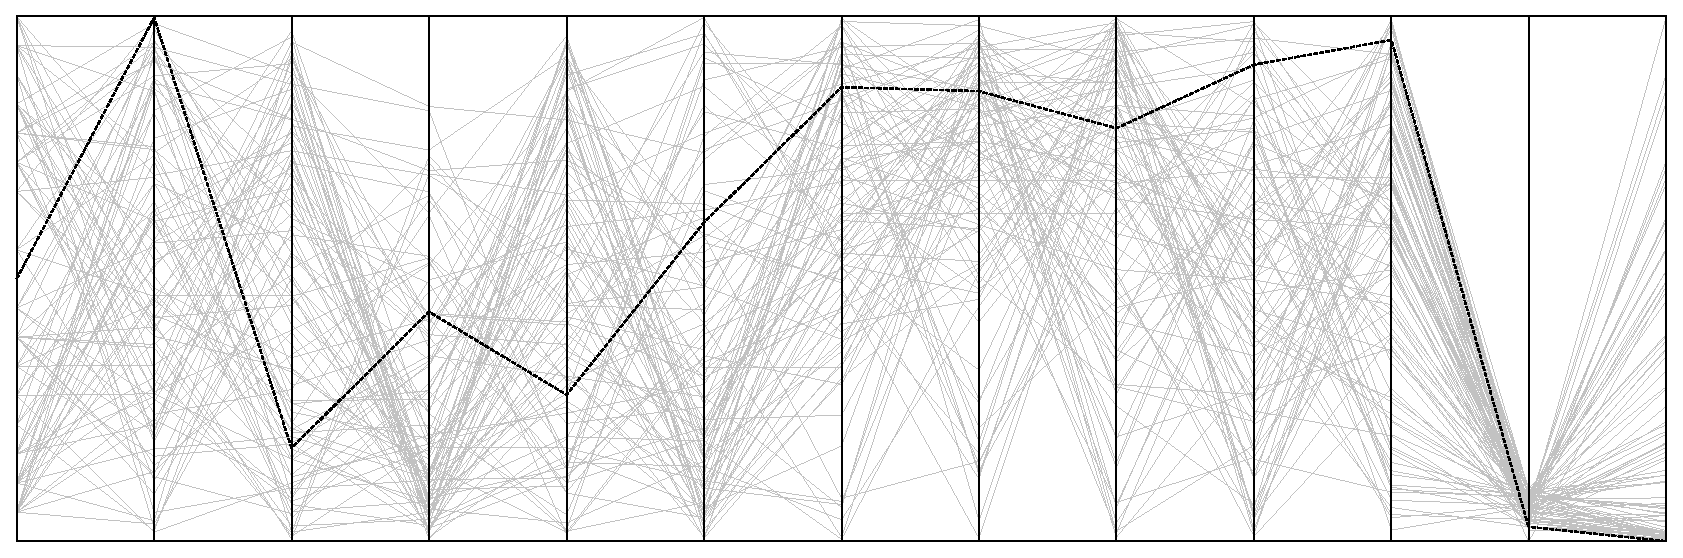
\includegraphics{sig_monks2_gnuplot_generalization}}%
    \gplfronttext
  \end{picture}%
\endgroup
